\documentclass{beamer}

\usepackage{amsmath}
\usepackage{amssymb}
\usepackage{mathtools}
%\usepackage{float}
\usepackage[pdftex]{graphicx}
%\usepackage[demo]{graphicx}
%\usepackage{ngerman}
\usepackage[T1]{fontenc}
\usepackage[utf8]{inputenc}
\usepackage{enumerate}
\usepackage{ifpdf}
\usetheme{Frankfurt}
\usecolortheme{default}
\usepackage[labelformat=empty]{caption}

\AtBeginSection[]
{
    \begin{frame}
        \frametitle{Übersicht}
        \tableofcontents[currentsection]
    \end{frame}
}

\title{Elektronikpraktikum Auswertung: Versuchstag 8} 
\subtitle{Analog/Digital-Wandlung}
\author{Gruppe 01 \\ Patrick Heuer \\ Benjamin Lotter}
\date{}

\begin{document}
\maketitle
\begin{frame}
    \frametitle{Übersicht}
    \tableofcontents
\end{frame}

\begin{frame}
\frametitle{Aufgabe 1}
\framesubtitle{Bestimmung von komplexem Widerstand und Phase}
    \begin{itemize}
        \item Bestimmung des Widerstands durch Messung von Strom und Spannung
        \item Strommessung = Spannungsmessung an bekanntem Widerstand
    \end{itemize}    
    \begin{figure}[H]
    \begin{center}
            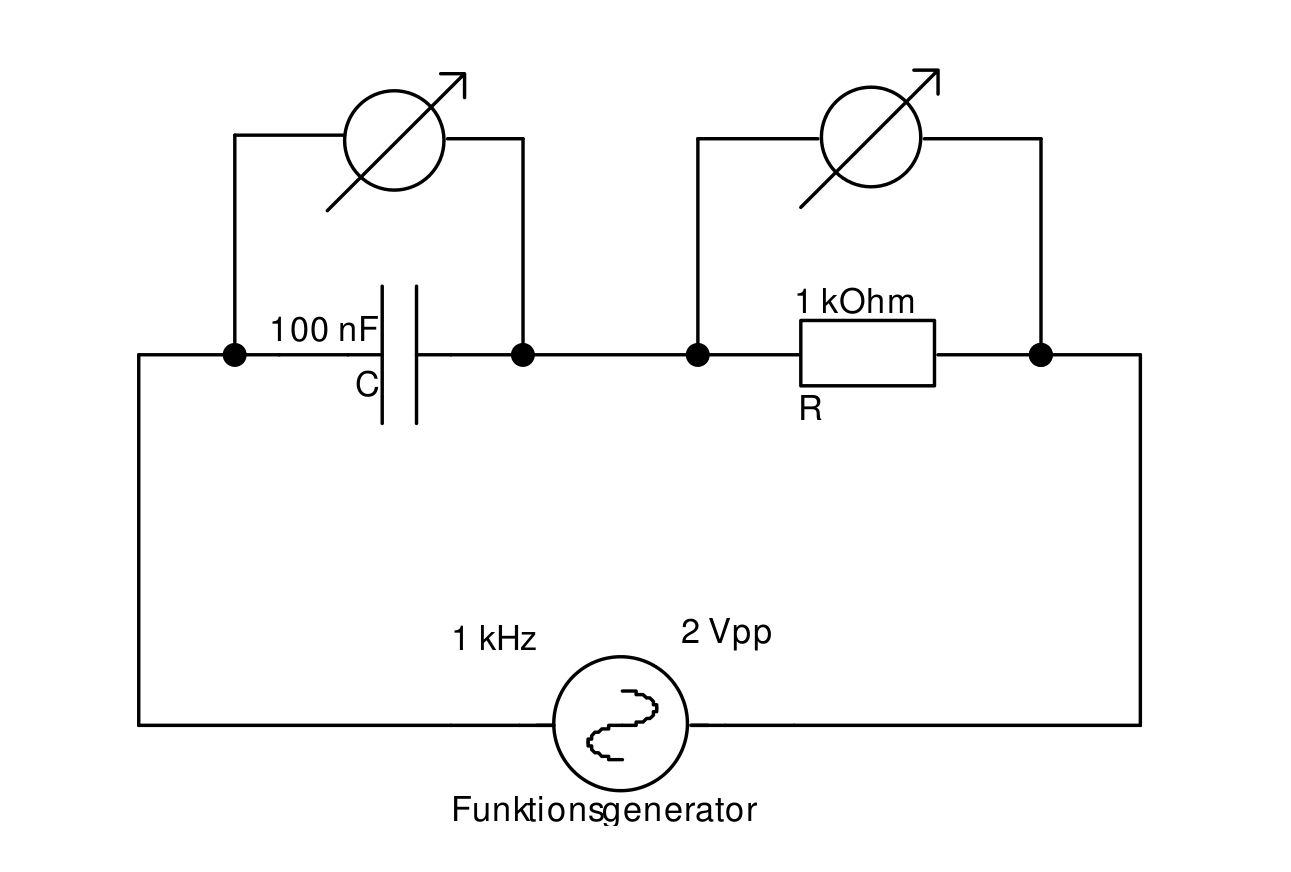
\includegraphics[scale=0.15]{./img/schaltbild_1_ohne_erdung.png}
    \end{center}
    \end{figure}
\end{frame}
\begin{frame}
\frametitle{Aufgabe 1}
\framesubtitle{Bestimmung von komplexem Widerstand und Phase}
    \begin{itemize}
        \item Problem: Erdschleife
    \end{itemize}
    \begin{figure}[H]
    \begin{center}
            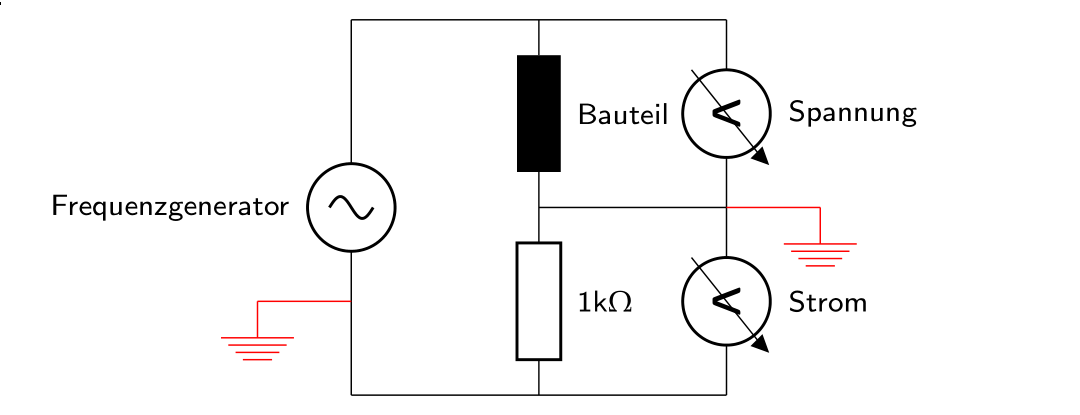
\includegraphics[scale=0.3]{./img/schaltbild_1_alle_erdungen.png}
    \end{center}
    \end{figure}
\end{frame}
\begin{frame}
\frametitle{Aufgabe 1}
\framesubtitle{Bestimmung von komplexem Widerstand und Phase}
    \begin{itemize}
        \item Problem: Erdschleife
        \item Lösung: Erdungen aufeinander legen
        \item Abfall über Bauteil: "Math function 2 - 1"
    \end{itemize}
    \begin{figure}[H]
    \begin{center}
            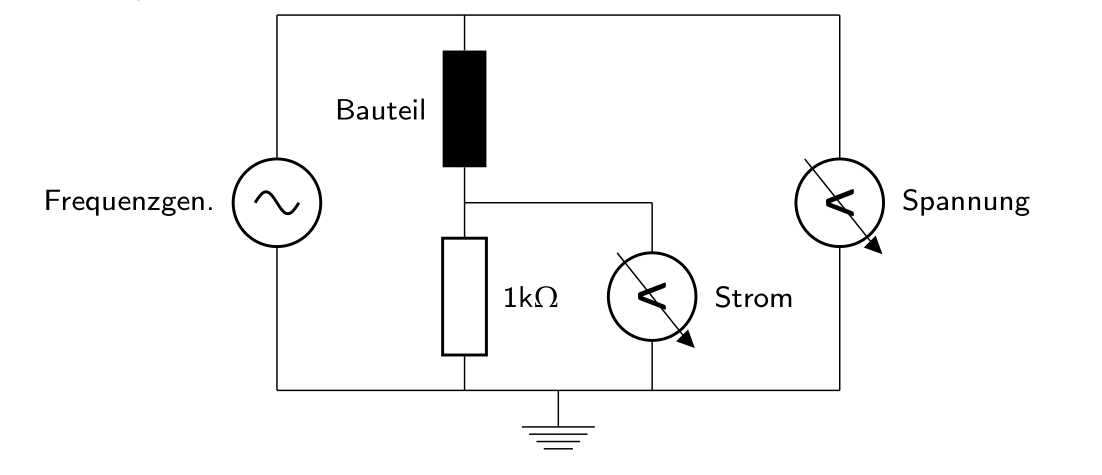
\includegraphics[scale=0.3]{./img/schaltbild_1_mit_erdschleife.png}
    \end{center}
    \end{figure}
\end{frame}

\begin{frame}
\frametitle{Aufgabe 1}
\framesubtitle{Kondensator}
\begin{figure}[H]
    \begin{center}
                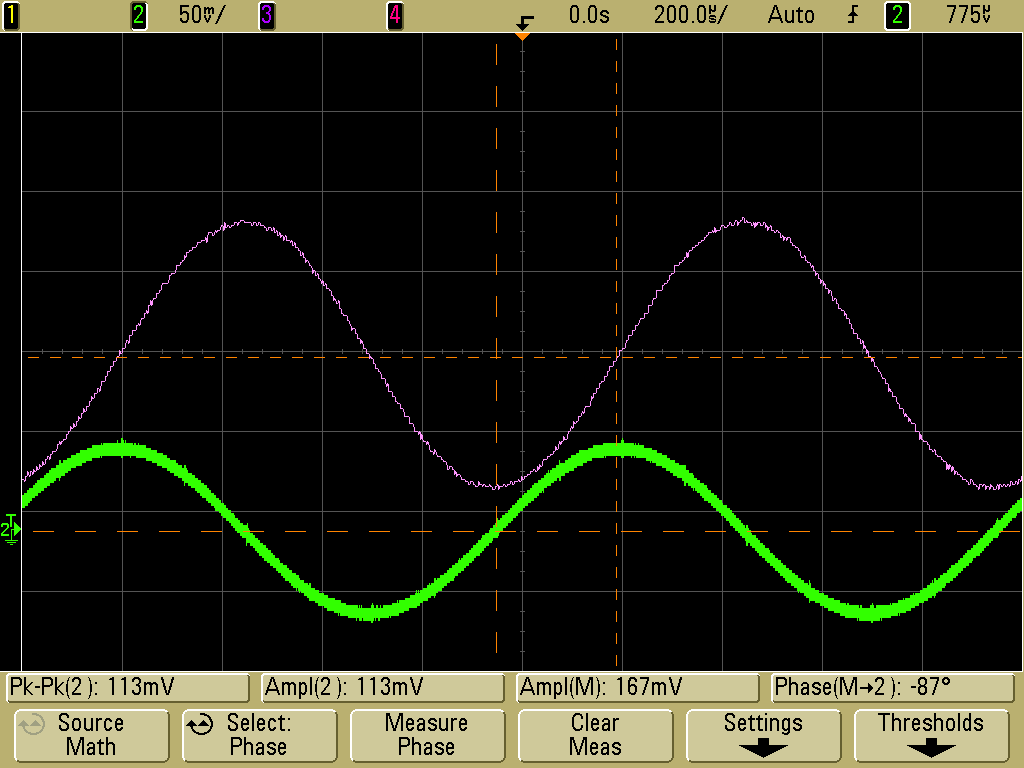
\includegraphics[scale=0.15]{./img/1a_Kondensator_1.png}
    \end{center}
\end{figure}
\begin{center}
\begin{tabular}{c|| c | c | c}
    & $I$ & $U$ & $\varphi$ \\
    \hline
    Kondensator ($100nF$)& $113 \mu A$ & $167mV$ & $-87^{\circ}$ \\
\end{tabular}
\end{center}
\end{frame}

\begin{frame}
\frametitle{Aufgabe 1}
\framesubtitle{Spule}
\begin{figure}[H]
    \begin{center}
                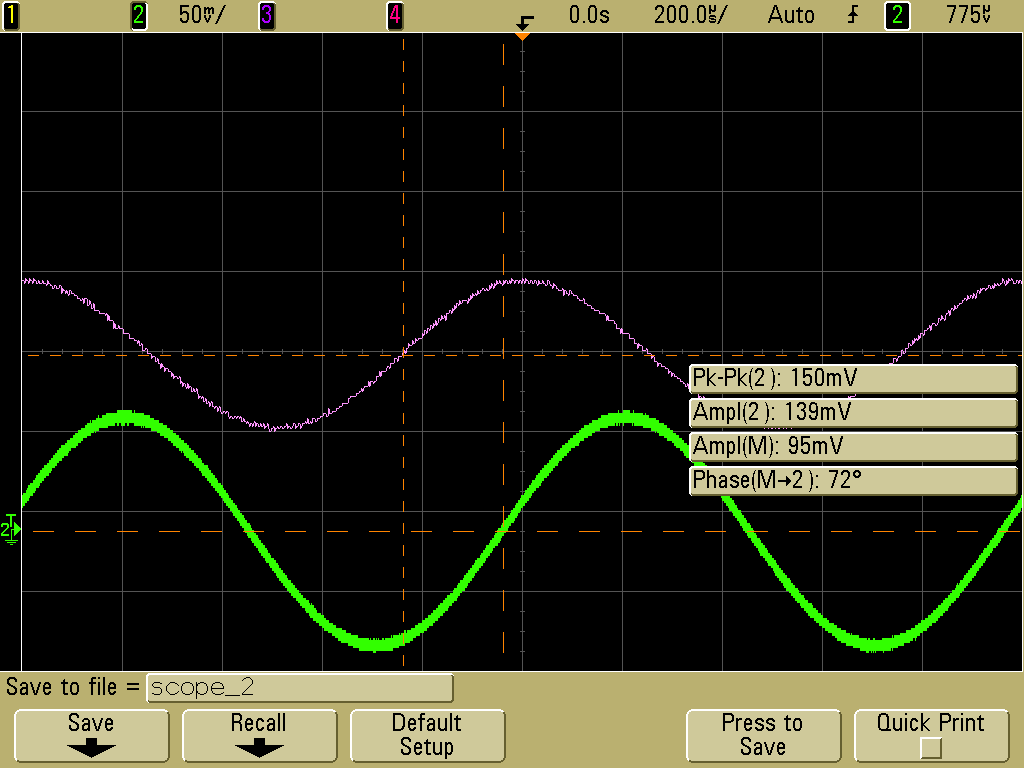
\includegraphics[scale=0.15]{./img/1b_Spule.png}
    \end{center}
\end{figure}
\begin{center}
\begin{tabular}{c|| c | c | c}
    & $I$ & $U$ & $\varphi$ \\
    \hline
    Kondensator ($100nF$)& $113 \mu A$ & $167mV$ & $-87^{\circ}$ \\
    Spule ($100mH$)& $139 \mu A$ & $95 mV$ & $72^{\circ}$ 
\end{tabular}
\end{center}
\end{frame}

\begin{frame}
\frametitle{Aufgabe 1}
\framesubtitle{Widerstand}
\begin{figure}[H]
    \begin{center}
                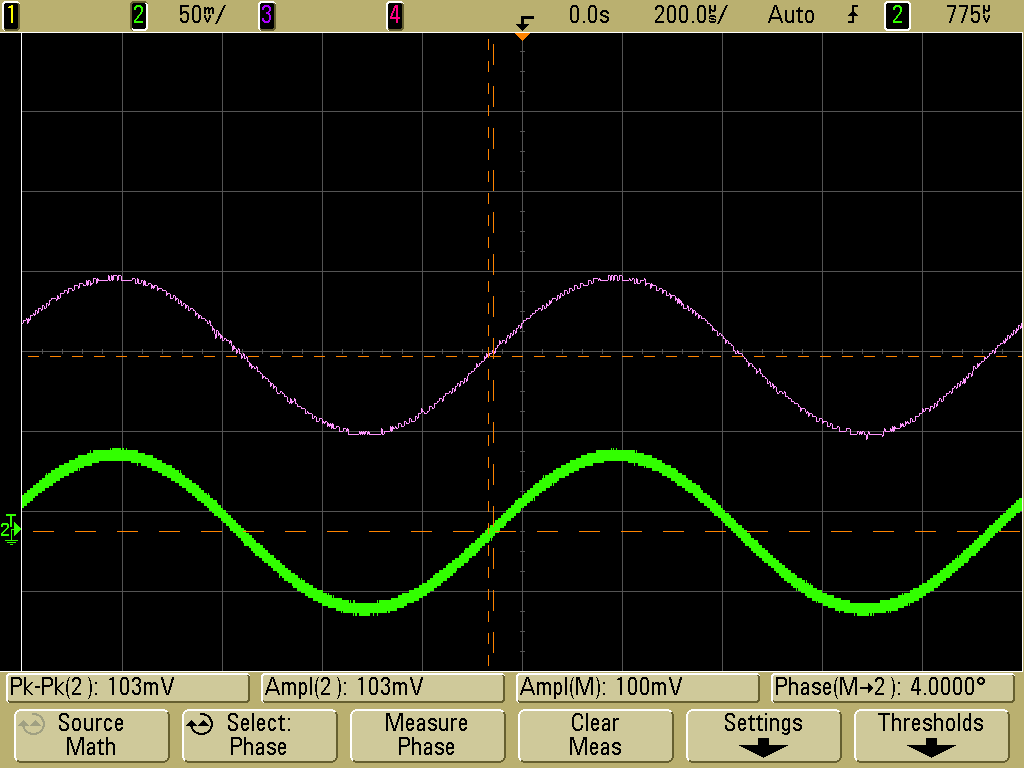
\includegraphics[scale=0.15]{./img/1c_Widerstand.png}
    \end{center}
\end{figure}
\begin{center}
\begin{tabular}{c|| c | c | c}
    & $I$ & $U$ & $\varphi$ \\
    \hline
    Kondensator ($100nF$)& $113 \mu A$ & $167mV$ & $-87^{\circ}$ \\
    Spule ($100mH$)& $139 \mu A$ & $95 mV$ & $72^{\circ}$  \\
    Widerstand ($1k\Omega$)& $104 \mu A$ & $100 mV$ & $4^{\circ}$
\end{tabular}
\end{center}
\end{frame}
\begin{frame}
\frametitle{Aufgabe 1}
\framesubtitle{Auswertung}
\begin{itemize}
    \item Komplexer Widerstand: $Z = \frac{U}{I} \left( \cos (\varphi) + i \sin
    (\varphi) \right) $
\end{itemize}
\begin{center}
\begin{tabular}{c|c|c}
    &   Messwert &  Theorie \\
    \hline
    $Z_C$ & $77.35 - i1475.85$ \Omega& $-i1592 \Omega$\\
    $Z_L$ & $211.20 + i650.00$ \Omega& $i629\Omega$ \\
    $Z_R$ & $968.51 - i 67.72$ \Omega& $1k\Omega$
\end{tabular}
\end{center}
\pause
\begin{itemize}
    \item $C = -i \frac{1}{2\pi f Z_C}$ und $L = \frac{Z_L}{i2\pi f}$:
\end{itemize}
\begin{align*}
    C &\approx 108 - i5.64nF \\
    L &\approx 103.45 - i33.61 mH
\end{align*}
\end{frame}
\begin{frame}
\frametitle{Aufgabe 1}
\framesubtitle{Auswertung}
\begin{center}
    \begin{tabular}{c|c|c}
        & Theorie & Messung \\
        \hline
        $\varphi_C$ & $-90^{\circ}$ & $-87^{\circ} $\\
        $\varphi_L$ & $90^{\circ}$ & $72^{\circ} $\\
        $\varphi_R$ & $0^{\circ}$ & $4^{\circ} $
    \end{tabular}
\end{center}
\begin{itemize}
    \item Gründe für Abweichung:
    \begin{itemize}
        \item ohmscher Widerstand der Bauteile
        \item Widerstand in Messgeräten
        \item Messungenauigkeit
    \end{itemize}
\end{itemize}
\end{frame}

\section{Analog-zu-Digital-Wandler (ADC)} % (fold)
\label{sec:Analog-zu-Digital-Wandler_(ADC}

\subsection{Erster Funktionstest} % (fold)
\label{sub:Erster Funktionstest}
\begin{frame}
\frametitle{Testsignalschaltung}
\framesubtitle{}
\begin{columns}[c]
    \column{0.65\textwidth}
         \begin{block}{$U_{in}$}
             \begin{itemize}
                \item $U_{in}$ liegt an Tiefpass:
                    \begin{equation*}
                        U_{in} = \frac{1}{\sqrt{\left(1+(R 2 \pi f
                        C)^2\right)}}\cdot U_{Fg} = 0.892V
                    \end{equation*}
                     für $f = 777Hz$,$U_{Fg} = 1V$
             \end{itemize}
         \end{block}
    \column{0.4\textwidth}
        \begin{figure}[H]
        \begin{center}
                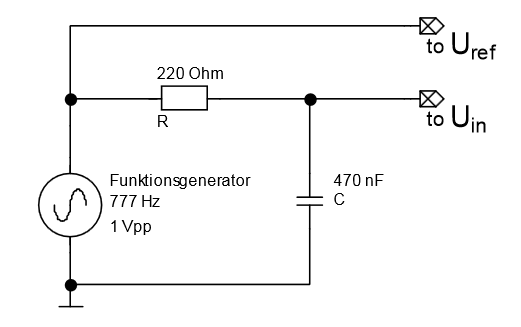
\includegraphics[scale=0.3]{./img/schaltung/testsignal.png}
        \end{center}
        \end{figure}
        \begin{figure}[H]
        \begin{center}
                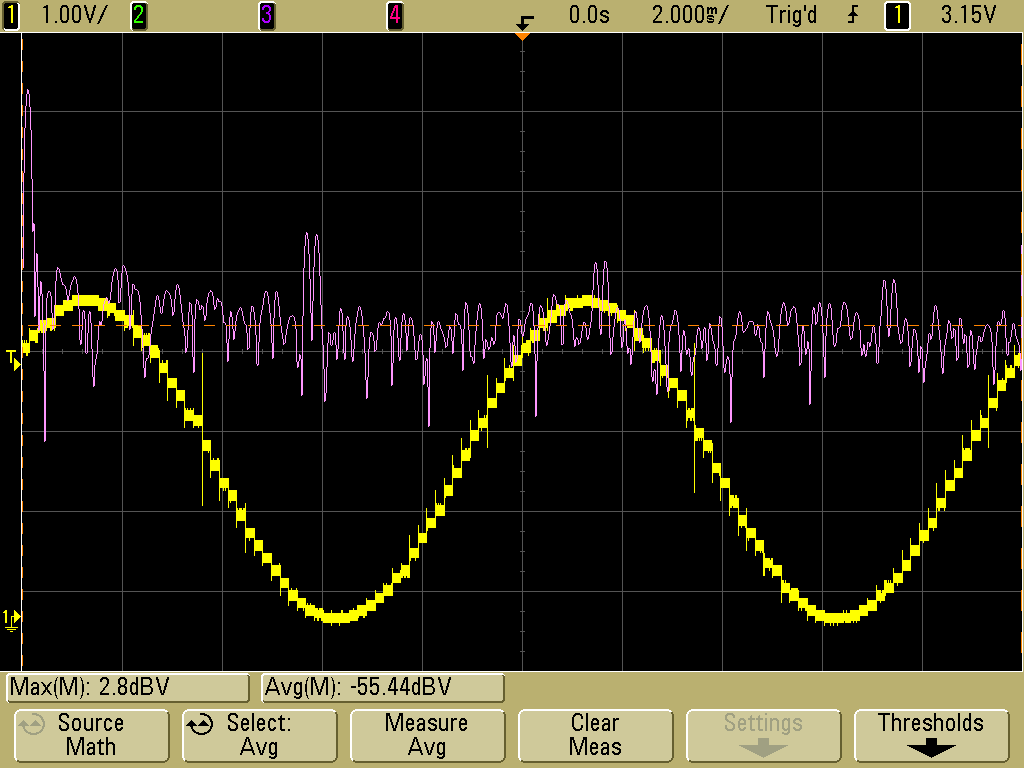
\includegraphics[scale=0.1]{./img/oszi/scope_21.png}
        \end{center}
        \end{figure}
        
        
\end{columns}

\end{frame}

\begin{frame}
\frametitle{Testsignalschaltung}
\framesubtitle{}
\begin{columns}[c]
    \column{0.65\textwidth}
         \begin{block}{Phase}
                 \begin{itemize}
                     \item Theoretische Phasenverschiebung:
                         \begin{equation*}
                             \varphi_{Th} = -\arctan{\left(2\pi f C R\right)} = 26.78^{\circ} 
                         \end{equation*}
                             für $f = 777Hz$
                    \item Gemessene Phasenverschiebung:
                        \begin{equation*}
                            \varphi_{Ge} = 21^{\circ}
                        \end{equation*}
                    \item
                        Mit $R_{Poti} = 6.96k\Omega$ bei maximalem $U_{out}$
                        ergibt sich eine Phasenverschiebung
                        \begin{equation*}
                            \varphi = 17.71^{\circ}
                        \end{equation*}
                 \end{itemize}
         \end{block}
    \column{0.4\textwidth}
        \begin{figure}[H]
        \begin{center}
                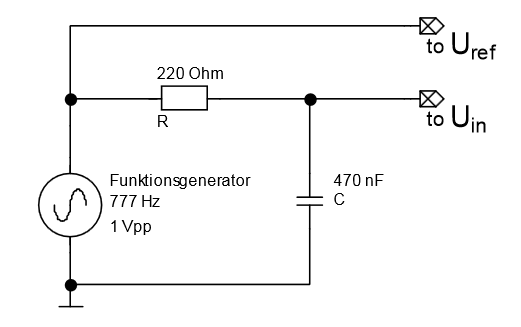
\includegraphics[scale=0.3]{./img/schaltung/testsignal.png}
        \end{center}
        \end{figure}
        \begin{figure}[H]
        \begin{center}
                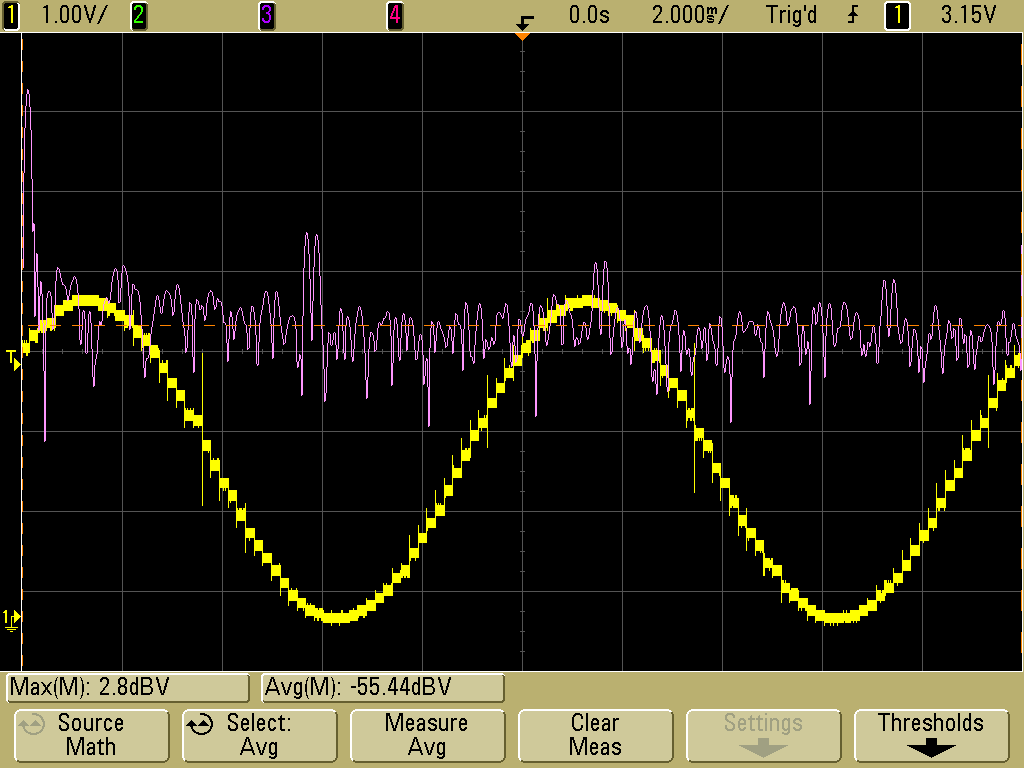
\includegraphics[scale=0.1]{./img/oszi/scope_21.png}
        \end{center}
        \end{figure}
\end{columns}
\end{frame}

\begin{frame}
    \frametitle{Messung}
    \framesubtitle{}
     \begin{figure}[H]
     \begin{center}
             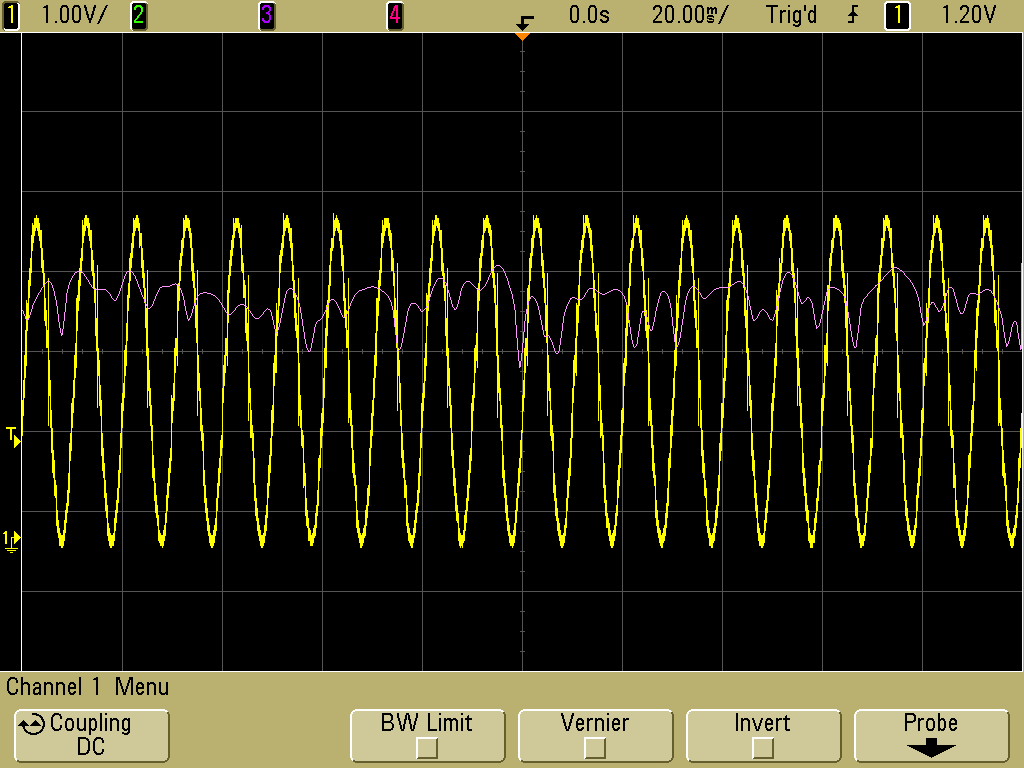
\includegraphics[scale=0.2]{./img/oszi/scope_18.png}
     \end{center}
     \caption{$U_{in}$ und $U_{ref}$ Phasenverschoben}
     \end{figure}
\end{frame}
\begin{frame}
    \frametitle{Messung}
    \framesubtitle{}
    \begin{figure}[H]
    \begin{center}
            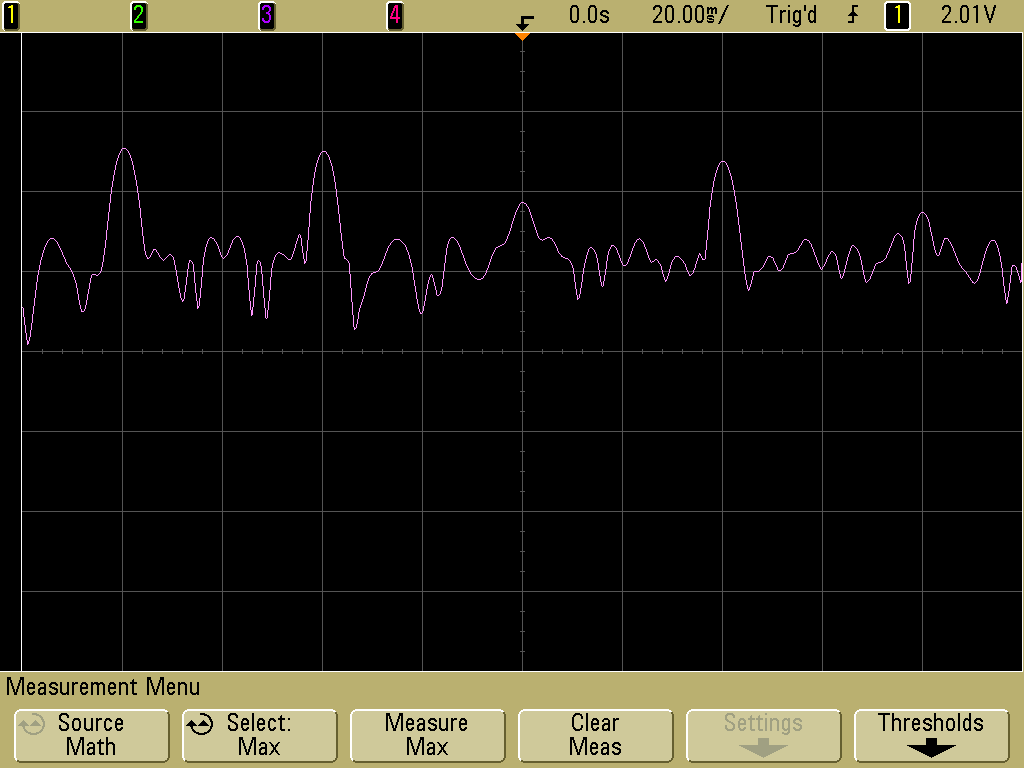
\includegraphics[scale=0.2]{./img/oszi/scope_17.png}
    \end{center}
     \caption{$U_{in}$ und $U_{ref}$ gleichphasig}
    \end{figure}
\end{frame}
% subsection Erster Funktionstest (end)

\subsection{Übertragung eines Lichtsignals} % (fold)
\label{sub:Übertragung eines Lichtsignals}
\begin{frame}
    \frametitle{Übertragung eines Lichtsignals}
    \framesubtitle{}
     \begin{columns}[c]
         \column{0.6\textwidth}
        \begin{block}{Ziel:}
             \begin{itemize}
                 \item Filterung der Störungen durch
                 \begin{itemize}
                     \item Lampen
                     \item Tageslicht
                 \end{itemize}
             \end{itemize}
        \end{block}
        \begin{block}{Versuch}
            \begin{itemize}
                \item moduliere LED-Signal mit $777Hz$ Spannung
                \item gebe Modulationsfrequenz als Referenzfrequenz weiter
                \item benutze L-I-Verstärker um $777Hz$ herauszufiltern
            \end{itemize}
        \end{block}
         \column{0.4\textwidth}
         \begin{figure}[H]
         \begin{center}
                 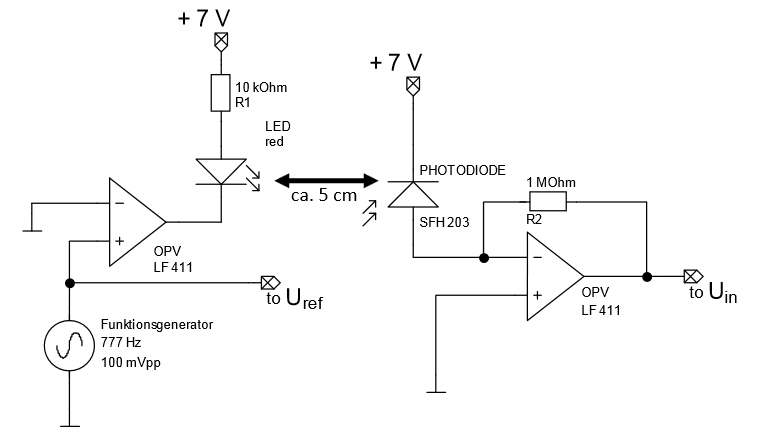
\includegraphics[scale=0.25]{./img/schaltung/optisch.png}
         \end{center}
         \end{figure}
     \end{columns}
\end{frame}

\begin{frame}
    \frametitle{Vergleich mit/ohne Abdeckung}
    \framesubtitle{}
    \begin{columns}[c]
        \column{0.5\textwidth}
        \begin{figure}[H]
        \begin{center}
                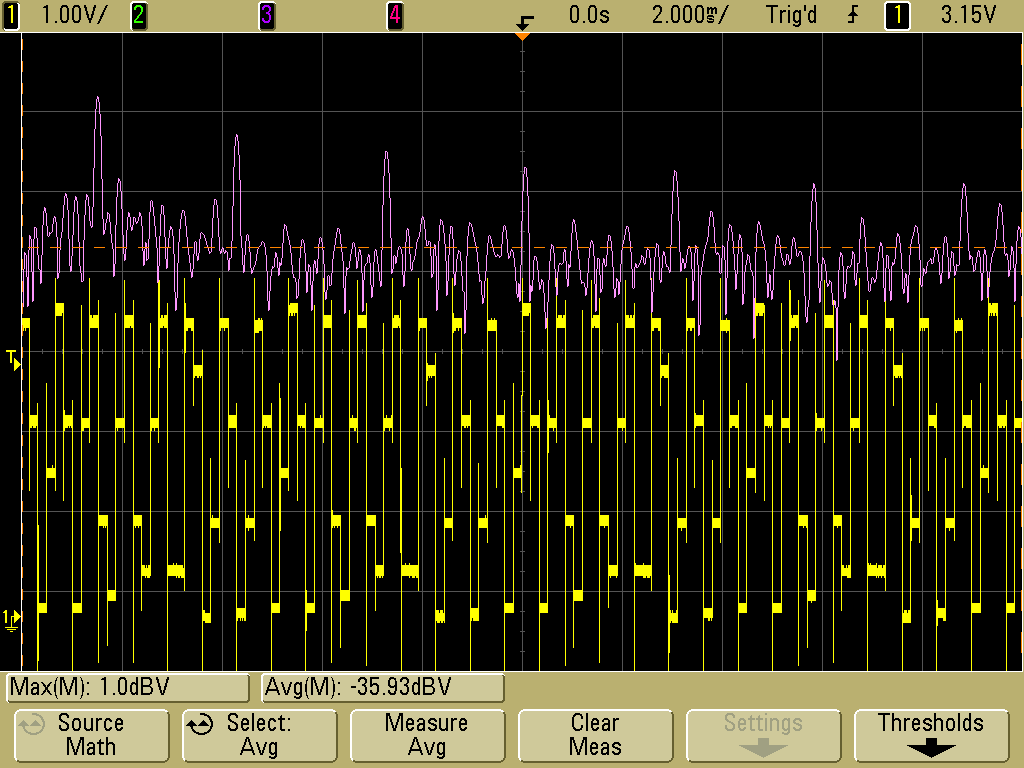
\includegraphics[scale=0.15]{./img/oszi/scope_23.png}
        \end{center}
        \caption{Ohne Abdeckung}
        \end{figure}
        \column{0.5\textwidth}
        \begin{figure}[H]
        \begin{center}
                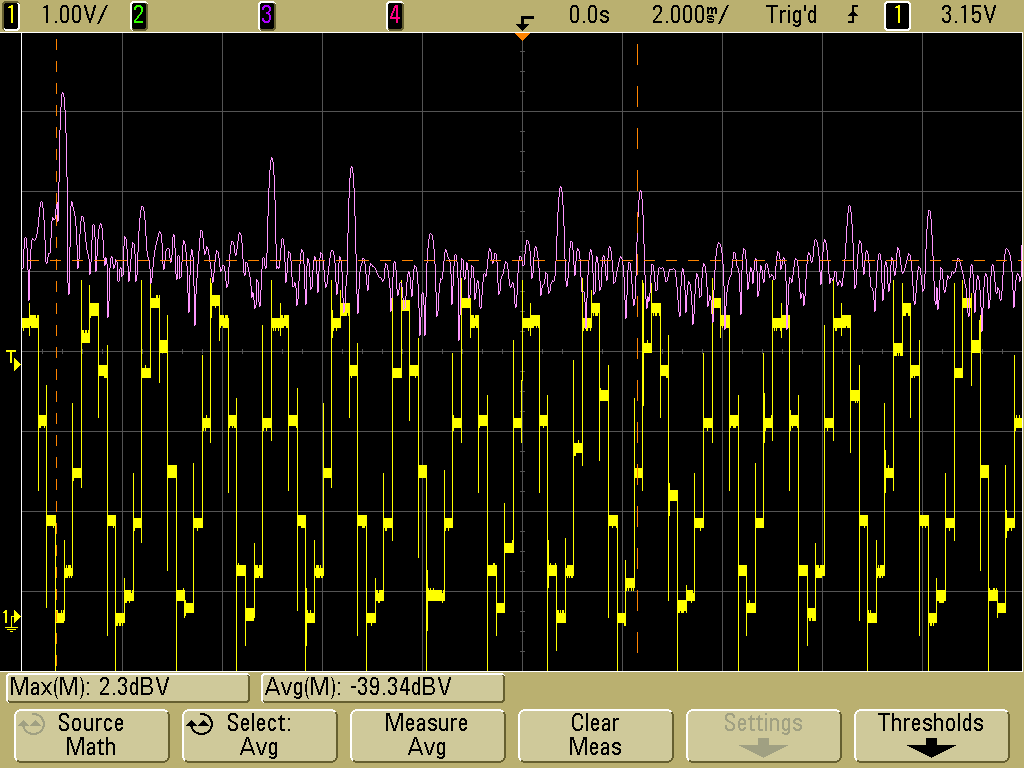
\includegraphics[scale=0.15]{./img/oszi/scope_22.png}
        \end{center}
        \caption{Mit Abdeckung}
        \end{figure}
    \end{columns}
        \begin{block}{}
            Ausgangssignal bleibt konstant auf $52.6mV$ $\rightarrow$ Schaltung
            filtert Störsignale heraus
        \end{block}
\end{frame}
% subsection Übertragung eines Lichtsignals (end)

% section Analog-zu-Digital-Wandler (ADC (end)

\section{Differenzverstärker} % (fold)
\label{sec:Differenzverstärker}
\begin{frame}
    \frametitle{Differenzverstärker}
    \framesubtitle{}
    \begin{block}{Ziel:}
        Verstärkung sehr kleiner Potentialunterschiede $\Delta V \approx 10\mu
        V$ \\ $\rightarrow$ Differenzverstärker
    \end{block}
    \pause
    \begin{figure}[H]
    \begin{center}
            \includegraphics[scale=0.2]{./img/schaltung/difver_1.png}
    \end{center}
    \end{figure}
\end{frame}
\begin{frame}
    \frametitle{Differenzverstärker}
    \framesubtitle{}
    
\end{frame}

% section Differenzverstärker (end)

\begin{frame}
\frametitle{Aufgabe 4}
\framesubtitle{}
    \begin{itemize}
        \item Durch kompliziertere Schaltungen können schärfere
        Frequenztrennungen erreicht werden
        \item Beim Tiefpass wurde fälschlicherweise eine Spule mit $L=100mH$
        verwendet
    \end{itemize}
\end{frame}
\begin{frame}
\frametitle{Aufgabe 4}
\framesubtitle{Tiefpass 2. Ordnung}
\begin{figure}[H]
\begin{center}
        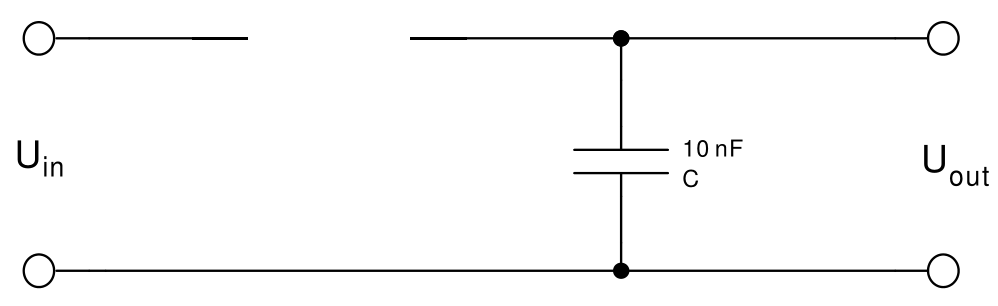
\includegraphics[scale=0.2]{./img/4a_tiefpass_1.png}
\end{center}
\end{figure}
\end{frame}
\begin{frame}
\frametitle{Aufgabe 4}
\framesubtitle{Tiefpass 2.Ordnung}
\begin{figure}[H]
\begin{center}
        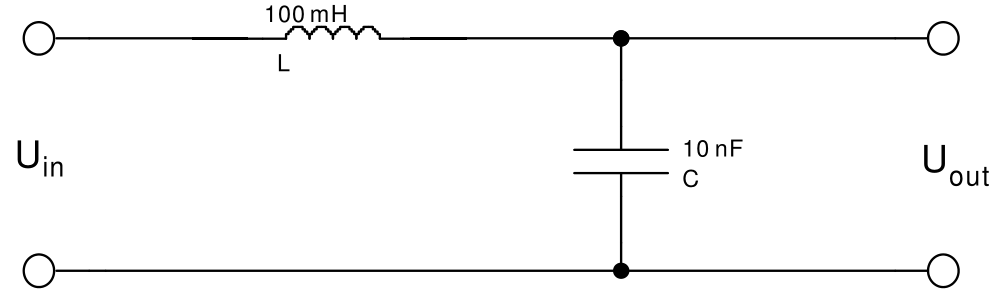
\includegraphics[scale=0.2]{./img/4a_tiefpass_2.png}
\end{center}
\end{figure}
\begin{itemize}
    \item Einbau von Spule
    \item Erwarteter Verlauf
\end{itemize}
\begin{equation*}
    \frac{U_{out}}{U_{in}} = \frac{1}{1-\omega^2 L C}
\end{equation*}
\end{frame}
\begin{frame}
\frametitle{Aufgabe 4}
\framesubtitle{Tiefpass Bode-Diagram}
    \begin{figure}[H]
    \begin{center}
            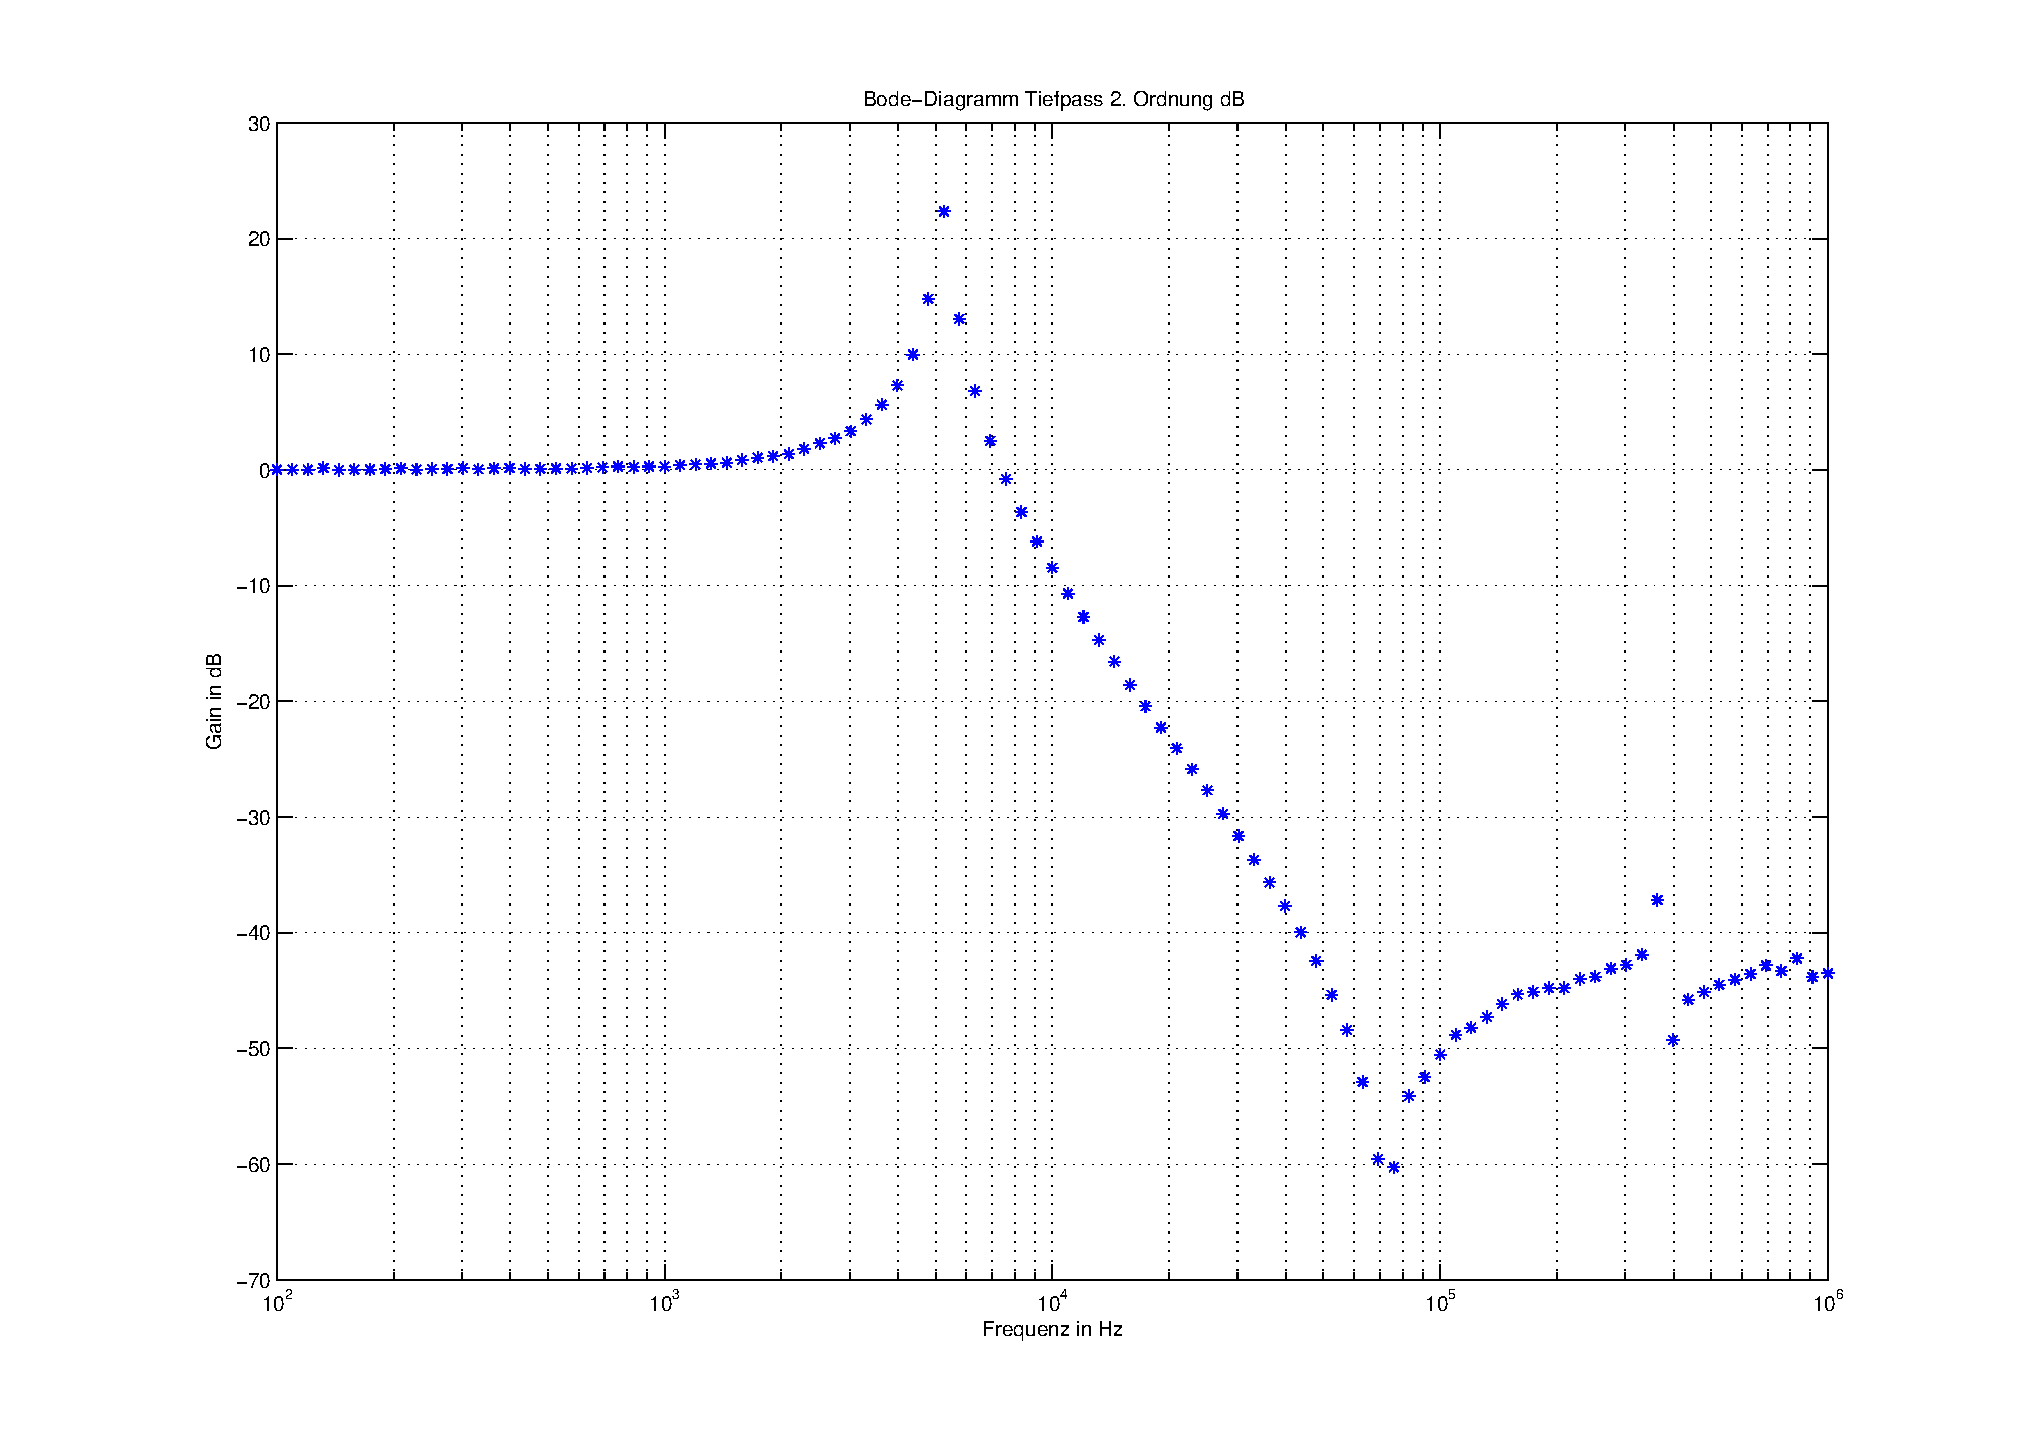
\includegraphics[scale=0.50]{./img/4a_bode_tief_dB.eps}
    \end{center}
    \end{figure}  
\begin{itemize}
    \item Unerwünschte Asymptote bei $\omega = \sqrt{\frac{1}{LC}}$
    \item Schwinkreis ohne Dämpfung
\end{itemize}
\end{frame}
\begin{frame}
    \frametitle{Aufgabe 4}
    \framesubtitle{Tiefpass mit Widerstand}
     %\begin{figure}[H]
     %\begin{center}
     %        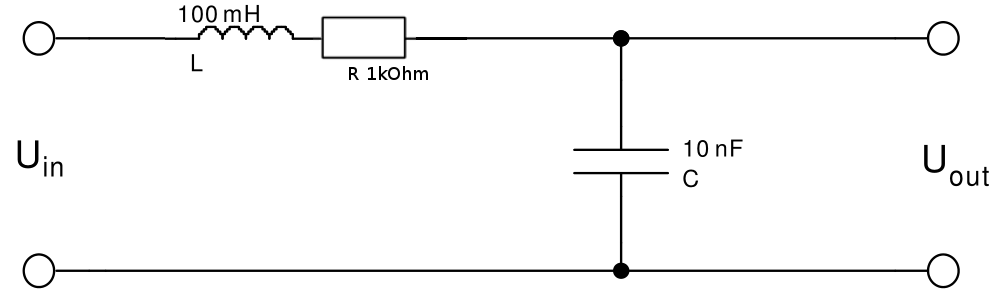
\includegraphics[scale=0.2]{4a_tiefpass_3.png}
     %\end{center}
     %\end{figure} 
     \begin{itemize}
        \item Zusätzlicher Widerstand
         \item Erwarteter Verlauf
     \end{itemize}
     \begin{equation*}
         \frac{U_{out}}{U_{in}}
         =
         \frac{Z_C}{Z_C + Z_L + R}
         =
         \frac{1}{\sqrt{\omega^4 L^2 C^2 + \omega^2 R^2 C^2 - 2 \omega^2 LC + 1}}
     \end{equation*}
\end{frame}
\begin{frame}
    \frametitle{Aufgabe 4}
    \framesubtitle{Tiefpass mit Widerstand}
     \begin{figure}[H]
     \begin{center}
             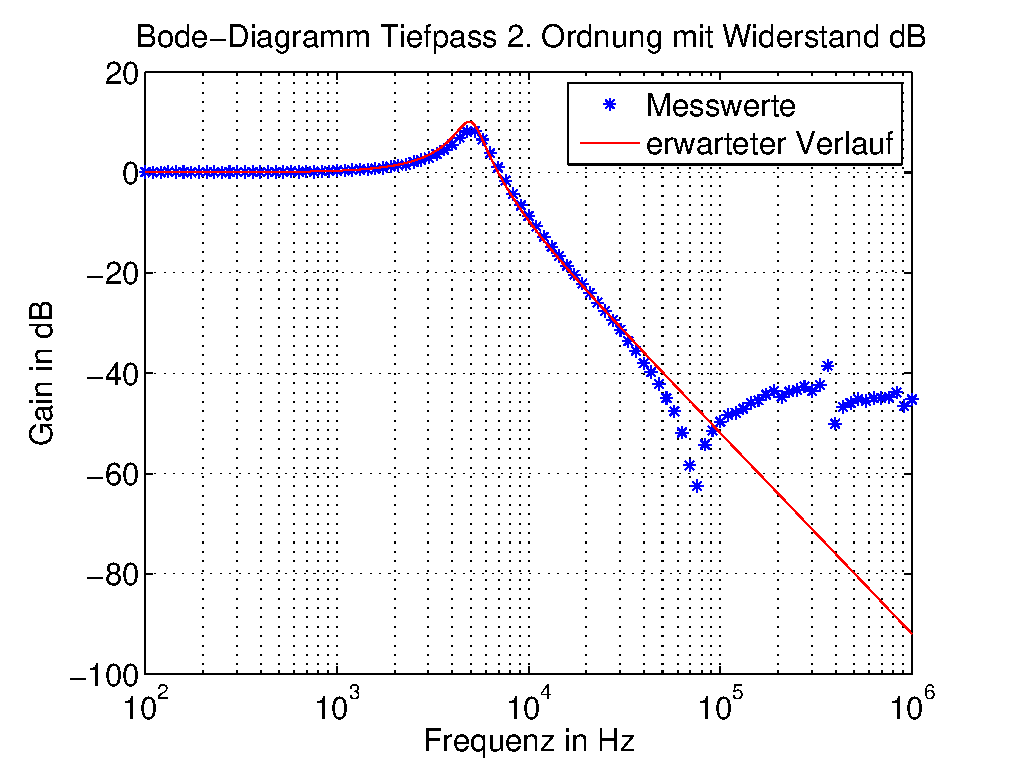
\includegraphics[scale=0.45]{./img/4a_bode_tief_dB_W.eps}
     \end{center}
     \end{figure}
     \begin{itemize}
        \item keine Asymptote
         \item Peak vor Abfall ist deutlich kleiner
         \item $R$ dämpft den Schwingkreis
     \end{itemize}
\end{frame}
\begin{frame}
    \frametitle{Aufgabe 4}
    \framesubtitle{Sperrkreisfilter}
    \begin{figure}[H]
    \begin{center}
            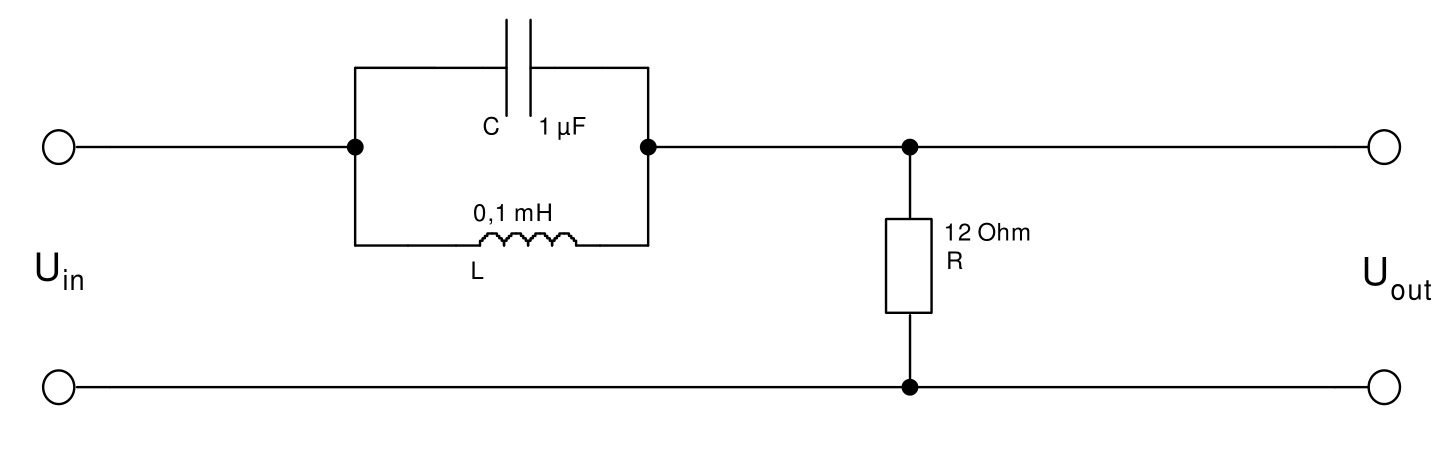
\includegraphics[scale=0.2]{./img/4b_schaltung.png}
    \end{center}
    \end{figure}
    \begin{equation*}
        \frac{U_{out}}{U_{in}}
        =
        \frac{\left\vert Z_R \right\vert}{\left\vert \frac{1}{\frac{1}{Z_C}+\frac{1}{Z_L}}
        +Z_R \right\vert }
        =
        \frac{R}{\sqrt{\left(\frac{\omega L}{\omega^2 C L +1}\right)^2 +
        R^2}}
    \end{equation*}
\end{frame}
\begin{frame}
    \frametitle{Aufgabe 4}
    \framesubtitle{Bode-Diagramm Sperrkreisfilter}
     \begin{figure}[H]
     \begin{center}
             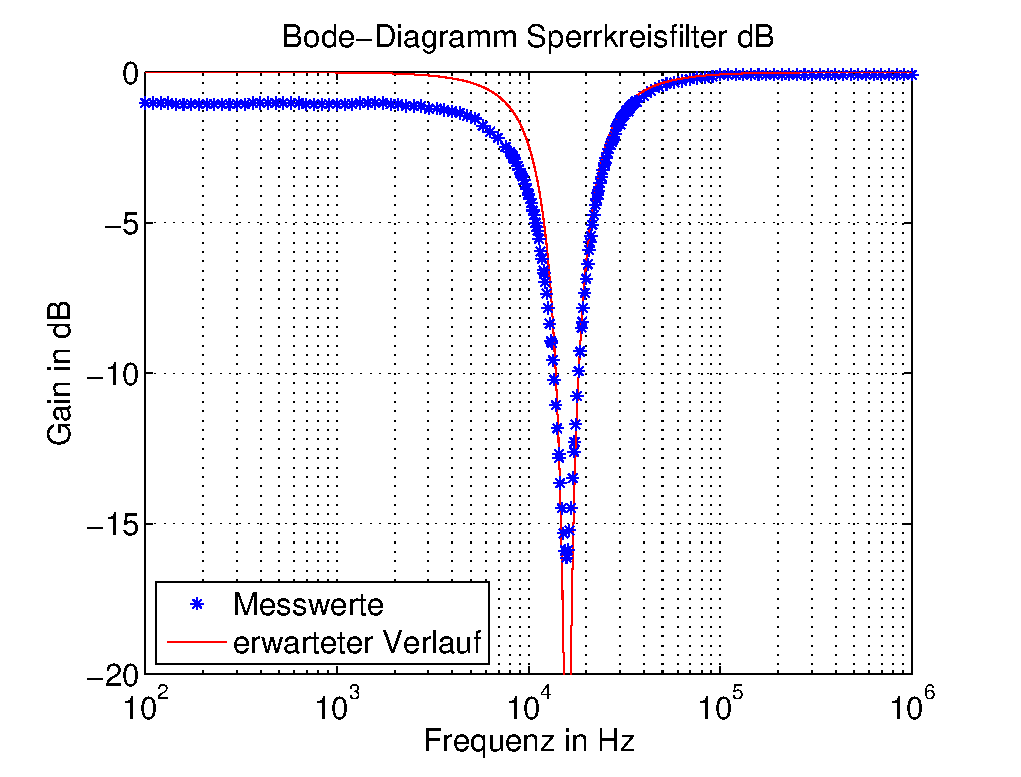
\includegraphics[scale=0.55]{./img/4b_dB.eps}
     \end{center}
     \end{figure}
\end{frame}
\begin{frame}
    \frametitle{Aufgabe 4}
    \framesubtitle{Bode-Diagramm Sperrkreisfilter}
     \begin{figure}[H]
     \begin{center}
             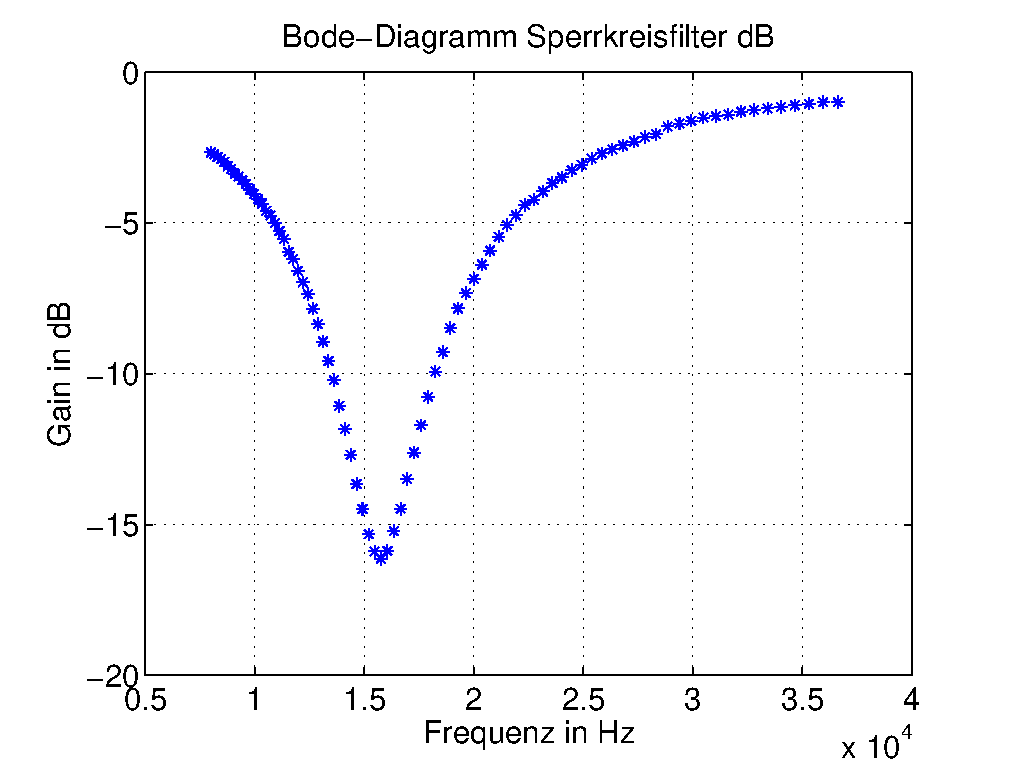
\includegraphics[scale=0.45]{./img/4b_Peak.eps}
     \end{center}
     \end{figure}
    \begin{itemize}
        \item Filtert einzelne Frequenz raus: $f \approx 16 kHz$
        \item Theorie: $f= \frac{1}{2\pi \sqrt{LC}}=15.91kHz$
    \end{itemize}
\end{frame}
\begin{frame}
    \frametitle{Aufgabe 4}
    \framesubtitle{Bode-Diagramm Sperrkreisfilter Phase}
     \begin{figure}[H]
     \begin{center}
             \includegraphics[scale=0.55]{./img/4b_Phase.eps}
     \end{center}
     \end{figure}
     \begin{itemize}
         \item Phase dreht sich beim Peak um
     \end{itemize}
\end{frame}


    
\end{document}
